%%%%%%%%%%%%%%%%%%%%%%%%%%%%%%%%%%%%%%%%%%%%%%%%%%%%%%%%%%%%%%%%%%%%%%%%%%%%%%%%
%2345678901234567890123456789012345678901234567890123456789012345678901234567890
%        1         2         3         4         5         6         7         8

\documentclass[letterpaper, 10 pt, conference]{ieeeconf}  % Comment this line out if you need a4paper
\usepackage[utf8]{inputenc}

\usepackage{authblk}
\usepackage{tabularx}
\usepackage{graphicx}
%\usepackage{gensymb}
\usepackage{siunitx}

%\documentclass[a4paper, 10pt, conference]{ieeeconf}      % Use this line for a4 paper

\IEEEoverridecommandlockouts                              % This command is only needed if
                                                          % you want to use the \thanks command

\overrideIEEEmargins                                      % Needed to meet printer requirements.

% See the \addtolength command later in the file to balance the column lengths
% on the last page of the document

% The following packages can be found on http:\\www.ctan.org
%\usepackage{graphics} % for pdf, bitmapped graphics files
%\usepackage{epsfig} % for postscript graphics files
%\usepackage{mathptmx} % assumes new font selection scheme installed
%\usepackage{times} % assumes new font selection scheme installed
%\usepackage{amsmath} % assumes amsmath package installed
%\usepackage{amssymb}  % assumes amsmath package installed

\title{\LARGE \bf
    Characterizing the Behavior of LiDARs in Snowy Conditions
}

\author[1]{Sébastien Michaud}
\author[2]{Jean-François Lalonde}
\author[1]{Philippe Giguère}

\affil[1]{Computer Science and Software Engineering, Laval University}
\affil[2]{Electrical and Computer Engineering, Laval University}


% \thanks{$^{1}$Sébastien Michaud is with Department of Computer Science and Software Engineering,
%         Laval University, 2325 Rue de l'Université, Québec, QC G1V 0A6, Canada
%         {\tt\small sebastien.michaud.2@ulaval.ca}}%
% \thanks{$^{2}$Jean-François Lalonde is with Department of Electrical and Computer Engineering,
%         Laval University, 2325 Rue de l'Université, Québec, QC G1V 0A6, Canada
%         {\tt\small jean-francois.lalonde@gel.ulaval.ca}}%
% \thanks{$^{3}$Philippe Giguère is with Department of Computer Science and Software Engineering,
%         Laval University, 2325 Rue de l'Université, Québec, QC G1V 0A6, Canada
%         {\tt\small philippe.giguere@ift.ulaval.ca}}%
% }

\begin{document}

\maketitle
\thispagestyle{empty}
\pagestyle{empty}

%!TEX root = ../root.tex
\begin{abstract}
Autonomous driving vehicles must be able to handle difficult weather conditions in order to gain acceptance. For example, challenging situations such as falling snow could significantly affect the performance of vision or LiDAR-based perception systems. In this paper, we are interested in characterizing the behavior of LiDARs in snowy conditions, as there seems to be little information publicly available. In particular, we present a characterization of the behavior of 4 commonly-used LiDARs (Velodyne HDL-32E, SICK LMS151, SICK LMS200 and Hokuyo UTM-30LX-EW) during the falling snow condition. Data was collected from the 4 sensors simultaneously during 10 snowfalls. Statistical analysis of these data sets indicates that these sensors can be modeled in a probabilistic manner, allowing the use of a Bayesian framework to improve robustness. Using data provided by the multi-echo LiDAR UTM-30LX-EW, we analyze the temporal evolution of snowstorms, in order to replicate their general behavior in simulation. 
\end{abstract}



%%!TEX root = ../root.tex
\section{Introduction}

The robustness of autonomous vehicles has increased prodigiously in the recent years. While long-range autonomous driving on the highway has been around for decades already~\cite{Pomerleau_1996_616}, advances in mapping, 3D data processing and computer vision have enabled cars to drive autonomously for thousands of miles in unconstrained, city environments~\cite{urmson2008autonomous}. While this surely is an impressive feat, one quickly notes that most of these miles have been logged in California weather, which provides optimal operating conditions for sensors such as LiDARs. In order for these systems to gain acceptance worldwide, it is crucial that they could be operated in more challenging weather conditions, such as rain, fog and snow. 

As we strive to make autonomous vehicles more adaptable to varying weather conditions, it is important to understand how sensors will behave in such conditions. Of particular interest, snowy conditions may cause challenging situations for sensors such as LiDARs. Indeed, the laser beams emitted may illuminate the snowflakes themselves, thus providing echoes that do not correspond to real obstacles. Consider fig.~\ref{fig:good-bad-weather} for example. The same scene appears drastically different depending on whether it was captured on a clear or snowy day. While programmable lighting may help circumvent this problem~\cite{tamburo2014programmable}, current LiDARs may fail under such circumstances. 

In this paper, our main contribution is to provide a characterization of the behavior of four well-known LiDARs in snowy conditions. Through an extensive empirical study performed on a novel dataset captured under varying degrees of snowfall, we evaluate how much these LiDARs are sensitive---or not---to falling snow. We show that recent advances in sensor design have increased their robustness even to significant snowfall. 

\begin{figure}
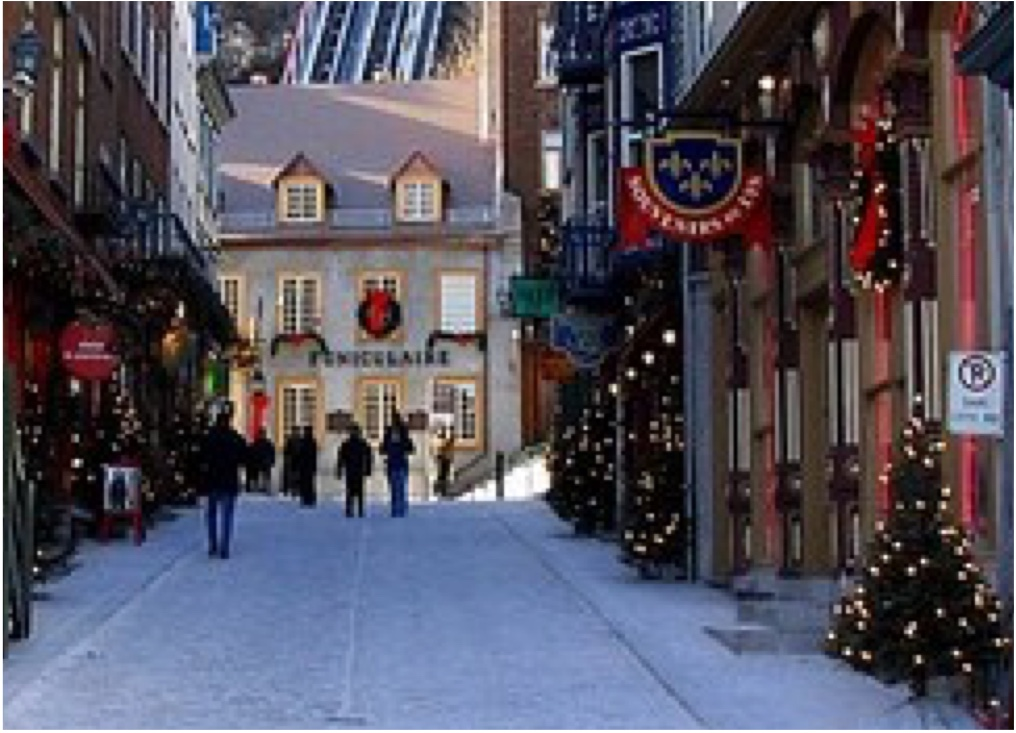
\includegraphics[width=.48\linewidth]{./img/teaser/summer.jpg}
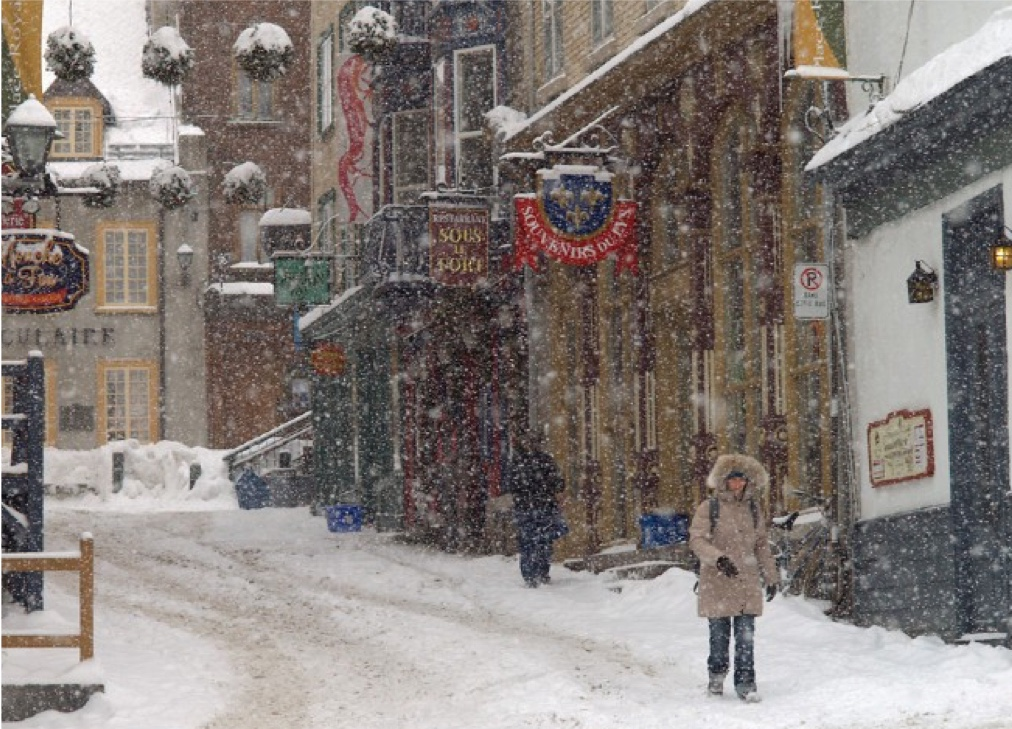
\includegraphics[width=.48\linewidth]{./img/teaser/winter.jpg}
\caption{Driving in bad weather. While autonomous vehicles have attained a great level of performance in nice weather (left), bad weather can cause significant challenges due to limited visibility (right). In this paper, we characterize the behavior in snowy conditions for oft-used sensors in autonomous cars: LiDARs. \emph{Photo credit}: Nicole Duchesne (left), Gaetan Chevalier (right).}
\label{fig:good-bad-weather}
\end{figure}

\subsection{Related work}

It is well-known that snow poses significant challenges to sensors mounted on-board outdoor mobile robots or other autonomous vehicles. For example, in their Antarctica exploration project, Moorehead et al. indicate that ``in heavy [snow] storms, [...] the laser could not be used''~\cite{Moorehead_1999_2122}. Similarly, Yamauchi et al. relate that ``LiDAR and stereo vision provide greater accuracy and resolution in clear weather but has difficulty with precipitation and obscurants''~\cite{yamauchi2010fusing}. Common approaches for dealing with this problem include filtering 3-D data~\cite{Moorehead_1999_2122}, or video~\cite{barnum2010analysis}, but this is often not enough to completely remove artifacts. 

It is therefore important to characterize how sensors behave in such conditions. To this end, Sumi et al.~\cite{sumi-arso-13} build a specifically designed simulated snow chamber, with white polystyrene beads flown with large fans to simulate snow. In our case, we use real world conditions to acquire a novel dataset of more than 6 days of snowfall.

Finally, we also mention the work of Servomaa et al.~\cite{servomaa2002snowfall}, who use LiDARs (and other sensors) to characterize snow storms for monitoring and measurement applications. In our case, we characterize the behavior of the sensors themselves for robotics applications.

% Less related: ground-penetrating radar to analyze polar ice-sheets~\cite{lever2013autonomous}. 



% autonomous vehicles more and more robust (cite efforts from Google/CMU/etc.)
% thousands of miles accumulated
% but in what weather? 

% as we strive to make autonomous vehicles more adaptable to various weather conditions, it's important to understand how sensors behave in such conditions. 
% of particular interest, snowy conditions may cause challenging situations for ... 
% show example of particularly bad snow scenes
% vision in bad weather (Srinivas) -- active lighting
% characterization of _real_ sensors, in _real_ snowy conditions, ranging from ... to ... 

% through a thorough analysis of this novel dataset, we show that most of the 3D sensors are indeed robust to significant snowfall (due to their own internal filtering algorithms), and that they're ok to work ``out of the box''. 


\section{Data Acquisition}

\subsection{Experimental Setup}
This section order : Sensors used + description, configuration of the sensors, scene + ground + shadow with figure of pictures seen from rgb camera.



Table~\ref{tab:lidars} show differents informations about the LiDARs. Note that all LiDARs use class 1 laser with a wavelength of \SI{905}{\nano\meter}.
\begin{table}[htbp]
    \centering
    \begin{tabularx}{\linewidth}{|X||c|c|}\hline
        Sensor              & Echoes     & Spot Shape \\ \hline%\hline
        Velodyne HDL-32E    & 1          & Rectangle  \\ \hline
        Hokuyo UTM-30LX-EW  & 3          & Ellipse    \\ \hline
        SICK LMS151         & 1 (second) & Circle     \\ \hline
        SICK LMS200         & 1          & Circle     \\ \hline
    \end{tabularx}
    \caption{LiDARs information}\label{tab:lidars}
\end{table}


 The sensors were placed close to the inner wall of a window facing N\SI{50}{\degree}E. A wooden structure held the LiDARs side by side at approximately \SI{13.9}{\meter} above the ground and the main scanning plane (i.e. \SI{0}{\degree} in the sensor reference frame) forming a \SI{30}{\degree} angle with respect to the building wall. In this configuration, a slight opening of the window allowed to keep the LiDARs inside while scanning outside. To avoid direct light exposure between sensors, corrugated plastic layers were placed between them. Note that we observed no interference between the sensor readings. Figure~\ref{fig:setup} present an overview of the setup.

\begin{figure}[h]
    \centering
    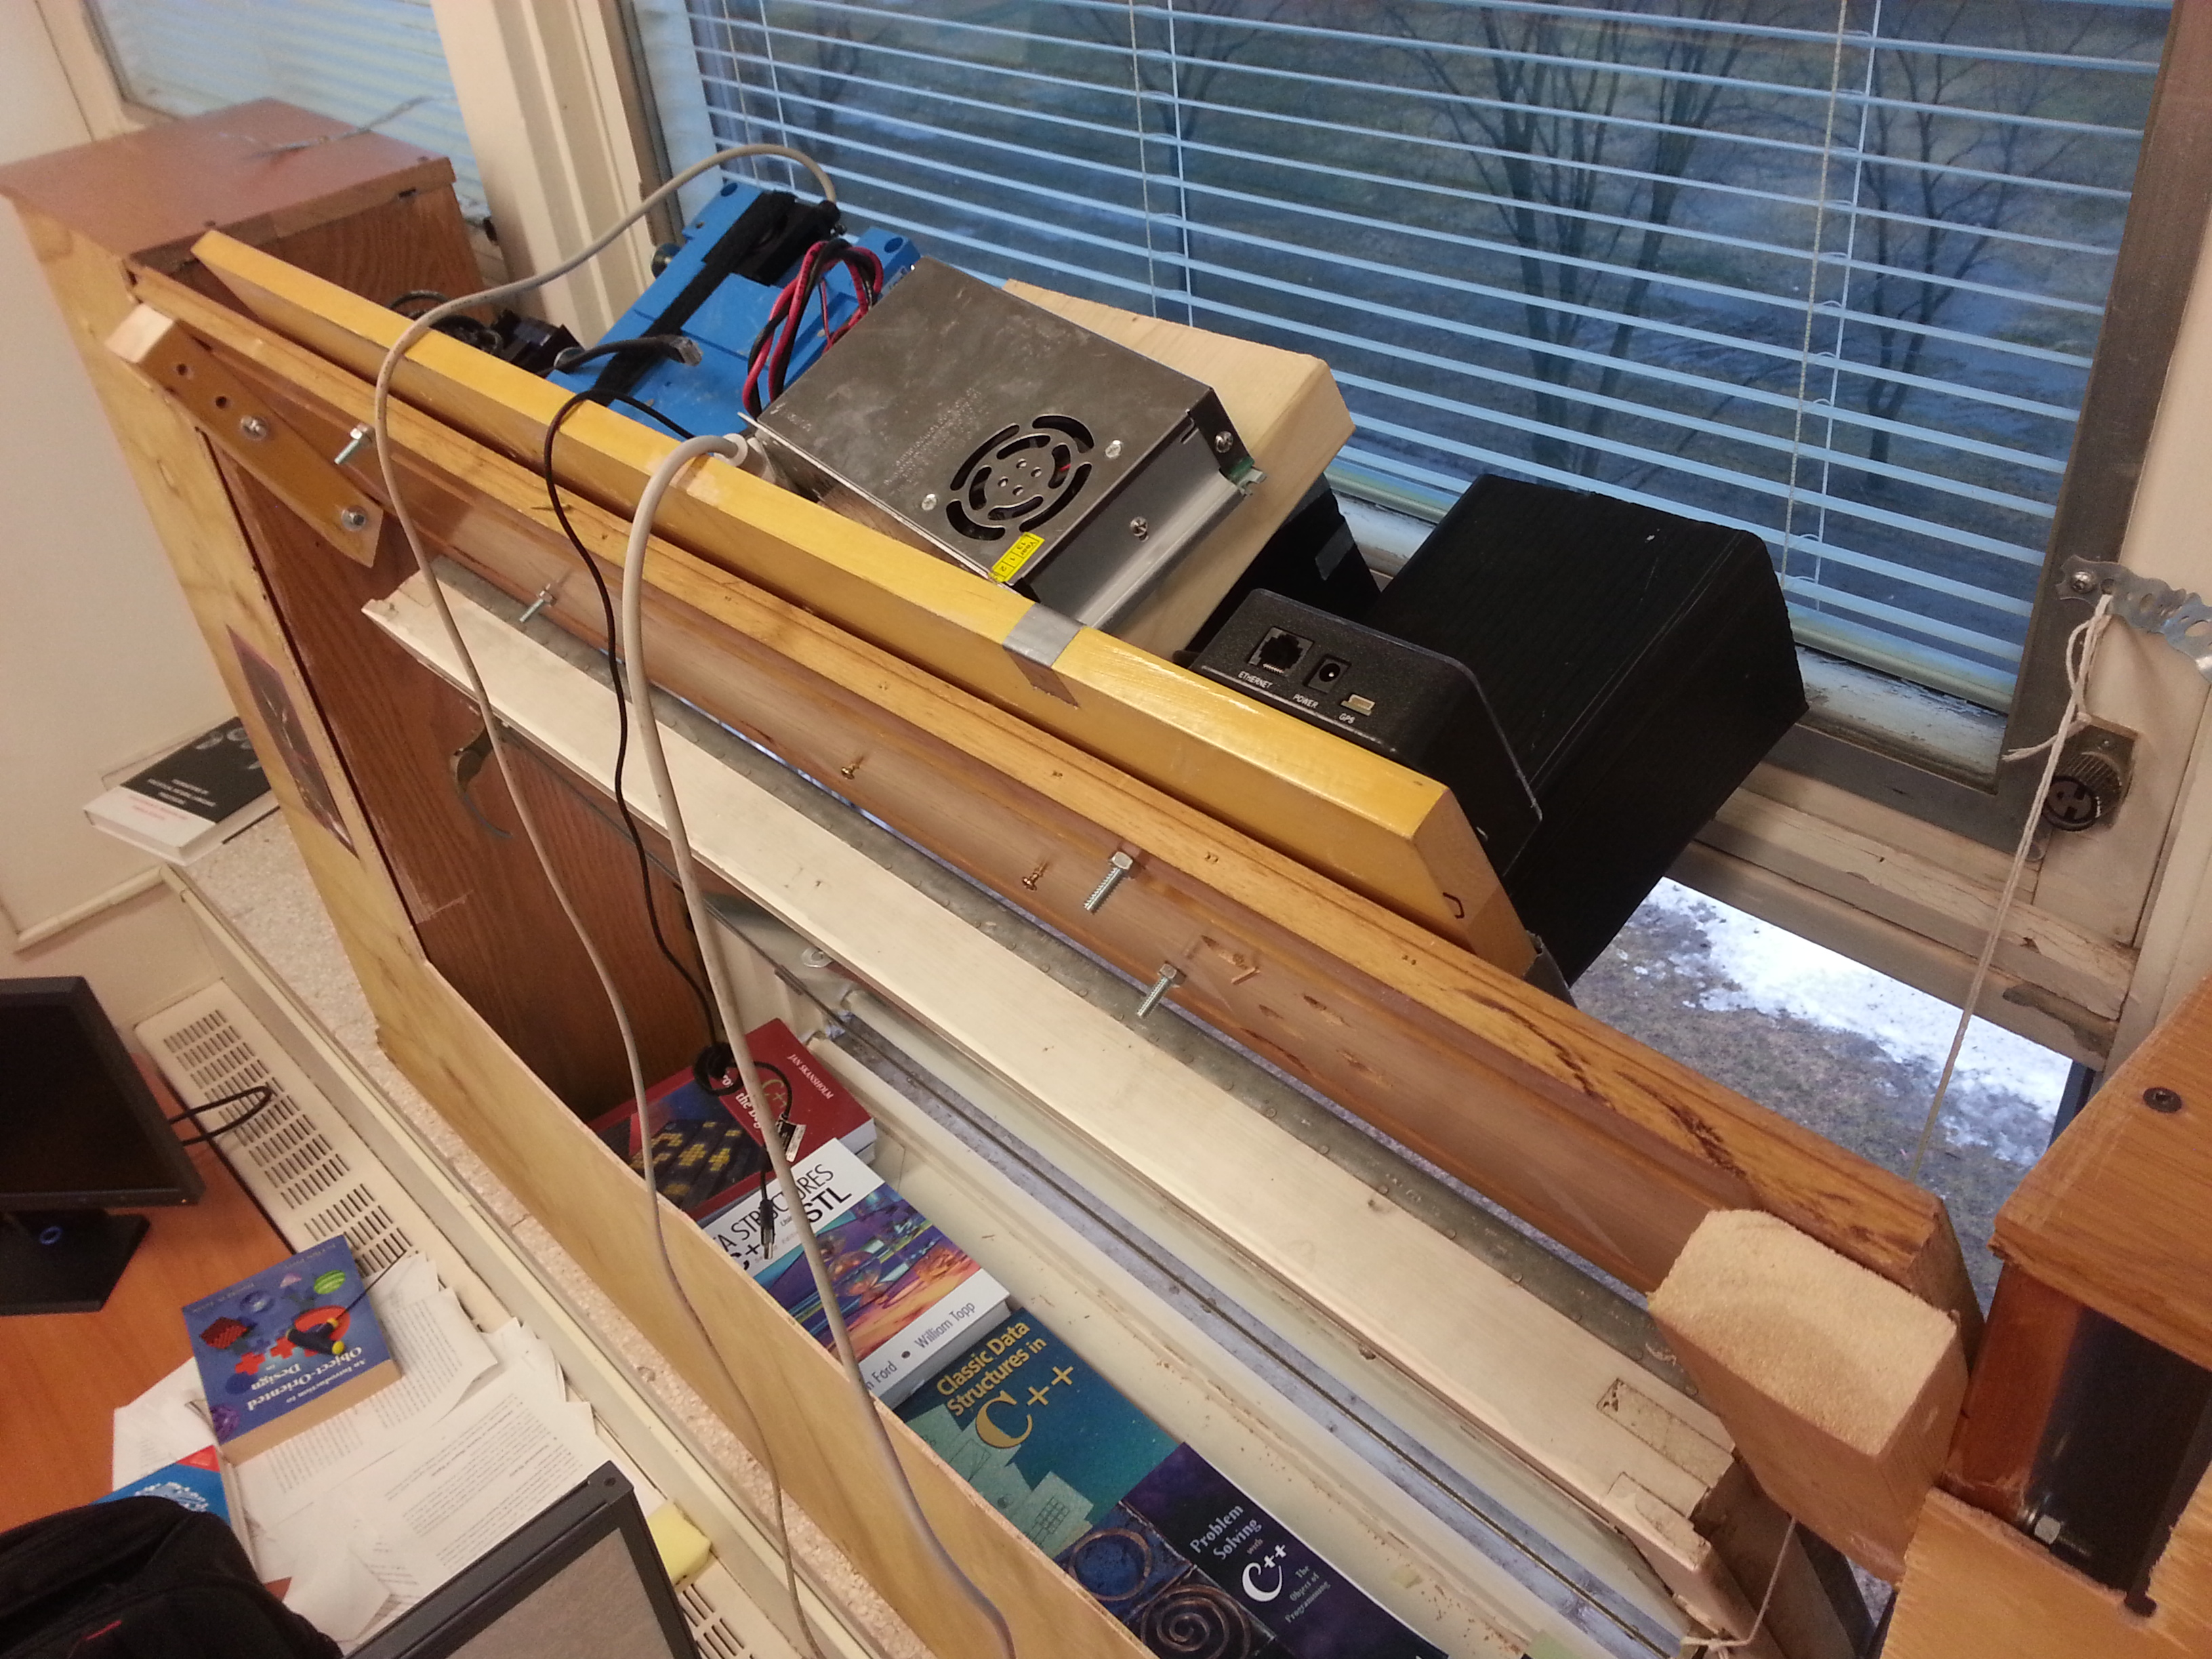
\includegraphics[width=0.95\linewidth]{./img/setup_diag.png}
    \caption{The experimental setup. The 3D axis represent the orientation of the sensors and the bottom left panel represent the 2D geometry as seen from the right side of the picture.}
    \label{fig:setup}
\end{figure}

\subsection{Dataset Description}
Describe the overall data (table that is in the google drive) in this section... Over a wide variety of temperature, cloudy not cloudy, different size of flakes windy...

Data acquisition was conducted at Pouliot Pavilion of Laval University beginning February 11 and ending March 21.

Recording of data was made through the Hydro distribution of the Robot Operating System (ROS)~\cite{ROSWeb}, which provide standardized data type as well as time synchronisation. The sicktoolbox\_wrapper~\cite{LMS200Web}, lms1xx~\cite{LMS151Web} and urg\_node~\cite{HokuyoWeb} packages provided \textit{LaserScan messages}\footnote{The LaserScan message definition is available at http://docs.ros.org/api/sensor\_msgs/html/msg/LaserScan.html} for the LMS200, LMS151 and UTM-30LX-EW respectively. The velodyne package~\cite{VelodyneWeb} produced the \textit{PointCloud2 messages}\footnote{The PointCloud2 message definition is available at http://docs.ros.org/api/sensor\_msgs/html/msg/PointCloud2.html} for the HDL-32E.

The orientation of the building relative to the sun cause a shadow on the ground where the...

\begin{figure}[h]
    \centering
    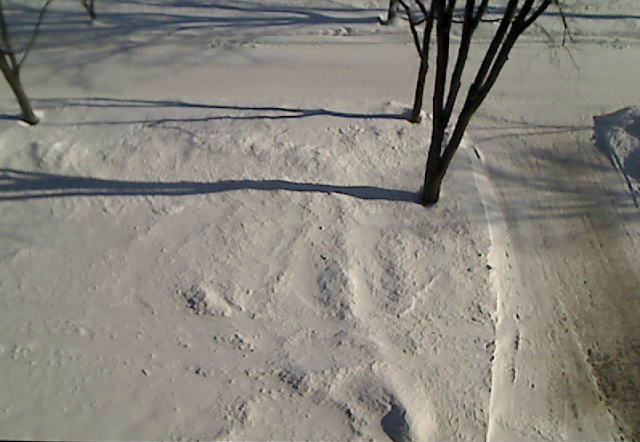
\includegraphics[width=0.90\linewidth]{./img/camera_view.jpg}
    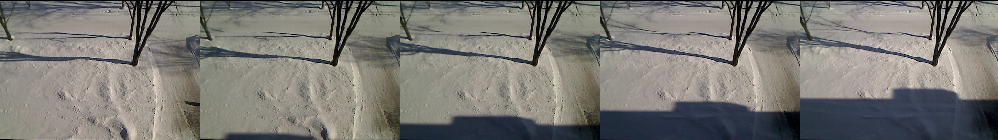
\includegraphics[width=0.95\linewidth]{./img/shadow2.png}
    \caption{View from the RGB camera. The sequence of pictures at the bottom shows the evolution of the shadow caused by the building between 10:00~am and 10:40~am.}
    \label{fig:setup}
\end{figure}

%Some notes to fill up the table:
%\begin{itemize}
    %\item LMS200
        %\begin{itemize}
            %\item See page 8. Range vs reflectivity
            %\item See page 7. It is around 20cm at 20m
        %\end{itemize}
    %\item LMS151
        %\begin{itemize}
            %\item See page 25. Scanning range up to 50 m (164.04 ft) with $>$ 75\% object remission (18 m (59.06 ft) with 10\% object remission)
            %\item See page 26. $distance(mm (in)) * 0.015 rad + 8 mm (0.31 in)$
        %\end{itemize}
    %\item Hokuyo
        %\begin{itemize}
            %\item 0.1 to 10m : $\pm$30mm,10 to 30m : $\pm$50mm(White Kent Sheet)
            %\item See article : Spot size is 50 mm × 500 mm at sensor’s maximum distance of 30 m
            %\item See page 6. Up to 3 echoes.
        %\end{itemize}
    %\item Velodyne
        %\begin{itemize}
            %\item See manual page 12. 1 to 70 meters... Datasheet says 80-100m...
            %\item See page 23. The lasers project a well defined rectangular shaped spot that is approximately 4” wide by 2” tall at 100’ distance. The spot size at the source of the HDL-32 is approximately 1/2” wide by 1/4” tall, causing the angular divergence to be 2.79 milliradians.
            %\item Time of flight
        %\end{itemize}
%\end{itemize}


%\section*{APPENDIX}
Appendixes should appear before the acknowledgment.


%\section*{ACKNOWLEDGMENT}
The preferred spelling of the word ÒacknowledgmentÓ in America is without an ÒeÓ after the ÒgÓ. Avoid the stilted expression, ÒOne of us (R. B. G.) thanks . . .Ó  Instead, try ÒR. B. G. thanksÓ. Put sponsor acknowledgments in the unnumbered footnote on the first page.



\end{document}
